\section{Ozone production}
\label{sec:ozone}

\subsection{Ozone generator setting}
\label{sec:ozone-setting}

The setup of the Ozone generator can be found in
Figure~\ref{fig:setup}. First we produce Zero Air by filtering lab air
through a carbon, a silica and then a particle filter. Afterwards we
irradiate the Zero Air with a Penra UV-lamp~\todo{find out more about
  lamp. Lines and stuff}. This produces the Ozone as seen in
Section~\ref{sec:theory}. The Zero Air was not cleansed of laughing
gas (\ch{N2O5}) which is not possible by a carbon nor a silica
filter. In the \SI{3}{\meter} teflon tube this laughing gas will react
with the Ozone and produce \ch{NO_x}, which then will be filtered by
the following silica gel. The gel filters Ozone, too, however, it
reaches its Ozone saturation level far quicker than its \ch{NO_x}
saturation level, thus after a short settling time the gel should not
hinder the Ozone. Afterwards we should have \ch{NO_x} free air
with a high concentration of Ozone.

\begin{figure}[htbp]
  \centering
  {
  \def\svgwidth{0.9\linewidth}
  %% Creator: Inkscape inkscape 0.91, www.inkscape.org
%% PDF/EPS/PS + LaTeX output extension by Johan Engelen, 2010
%% Accompanies image file 'setup.pdf_tex.pdf' (pdf, eps, ps)
%%
%% To include the image in your LaTeX document, write
%%   \input{<filename>.pdf_tex}
%%  instead of
%%   \includegraphics{<filename>.pdf}
%% To scale the image, write
%%   \def\svgwidth{<desired width>}
%%   \input{<filename>.pdf_tex}
%%  instead of
%%   \includegraphics[width=<desired width>]{<filename>.pdf}
%%
%% Images with a different path to the parent latex file can
%% be accessed with the `import' package (which may need to be
%% installed) using
%%   \usepackage{import}
%% in the preamble, and then including the image with
%%   \import{<path to file>}{<filename>.pdf_tex}
%% Alternatively, one can specify
%%   \graphicspath{{<path to file>/}}
%% 
%% For more information, please see info/svg-inkscape on CTAN:
%%   http://tug.ctan.org/tex-archive/info/svg-inkscape
%%
\begingroup%
  \makeatletter%
  \providecommand\color[2][]{%
    \errmessage{(Inkscape) Color is used for the text in Inkscape, but the package 'color.sty' is not loaded}%
    \renewcommand\color[2][]{}%
  }%
  \providecommand\transparent[1]{%
    \errmessage{(Inkscape) Transparency is used (non-zero) for the text in Inkscape, but the package 'transparent.sty' is not loaded}%
    \renewcommand\transparent[1]{}%
  }%
  \providecommand\rotatebox[2]{#2}%
  \ifx\svgwidth\undefined%
    \setlength{\unitlength}{1567.76523438bp}%
    \ifx\svgscale\undefined%
      \relax%
    \else%
      \setlength{\unitlength}{\unitlength * \real{\svgscale}}%
    \fi%
  \else%
    \setlength{\unitlength}{\svgwidth}%
  \fi%
  \global\let\svgwidth\undefined%
  \global\let\svgscale\undefined%
  \makeatother%
  \begin{picture}(1,0.56250002)%
    \put(0,0){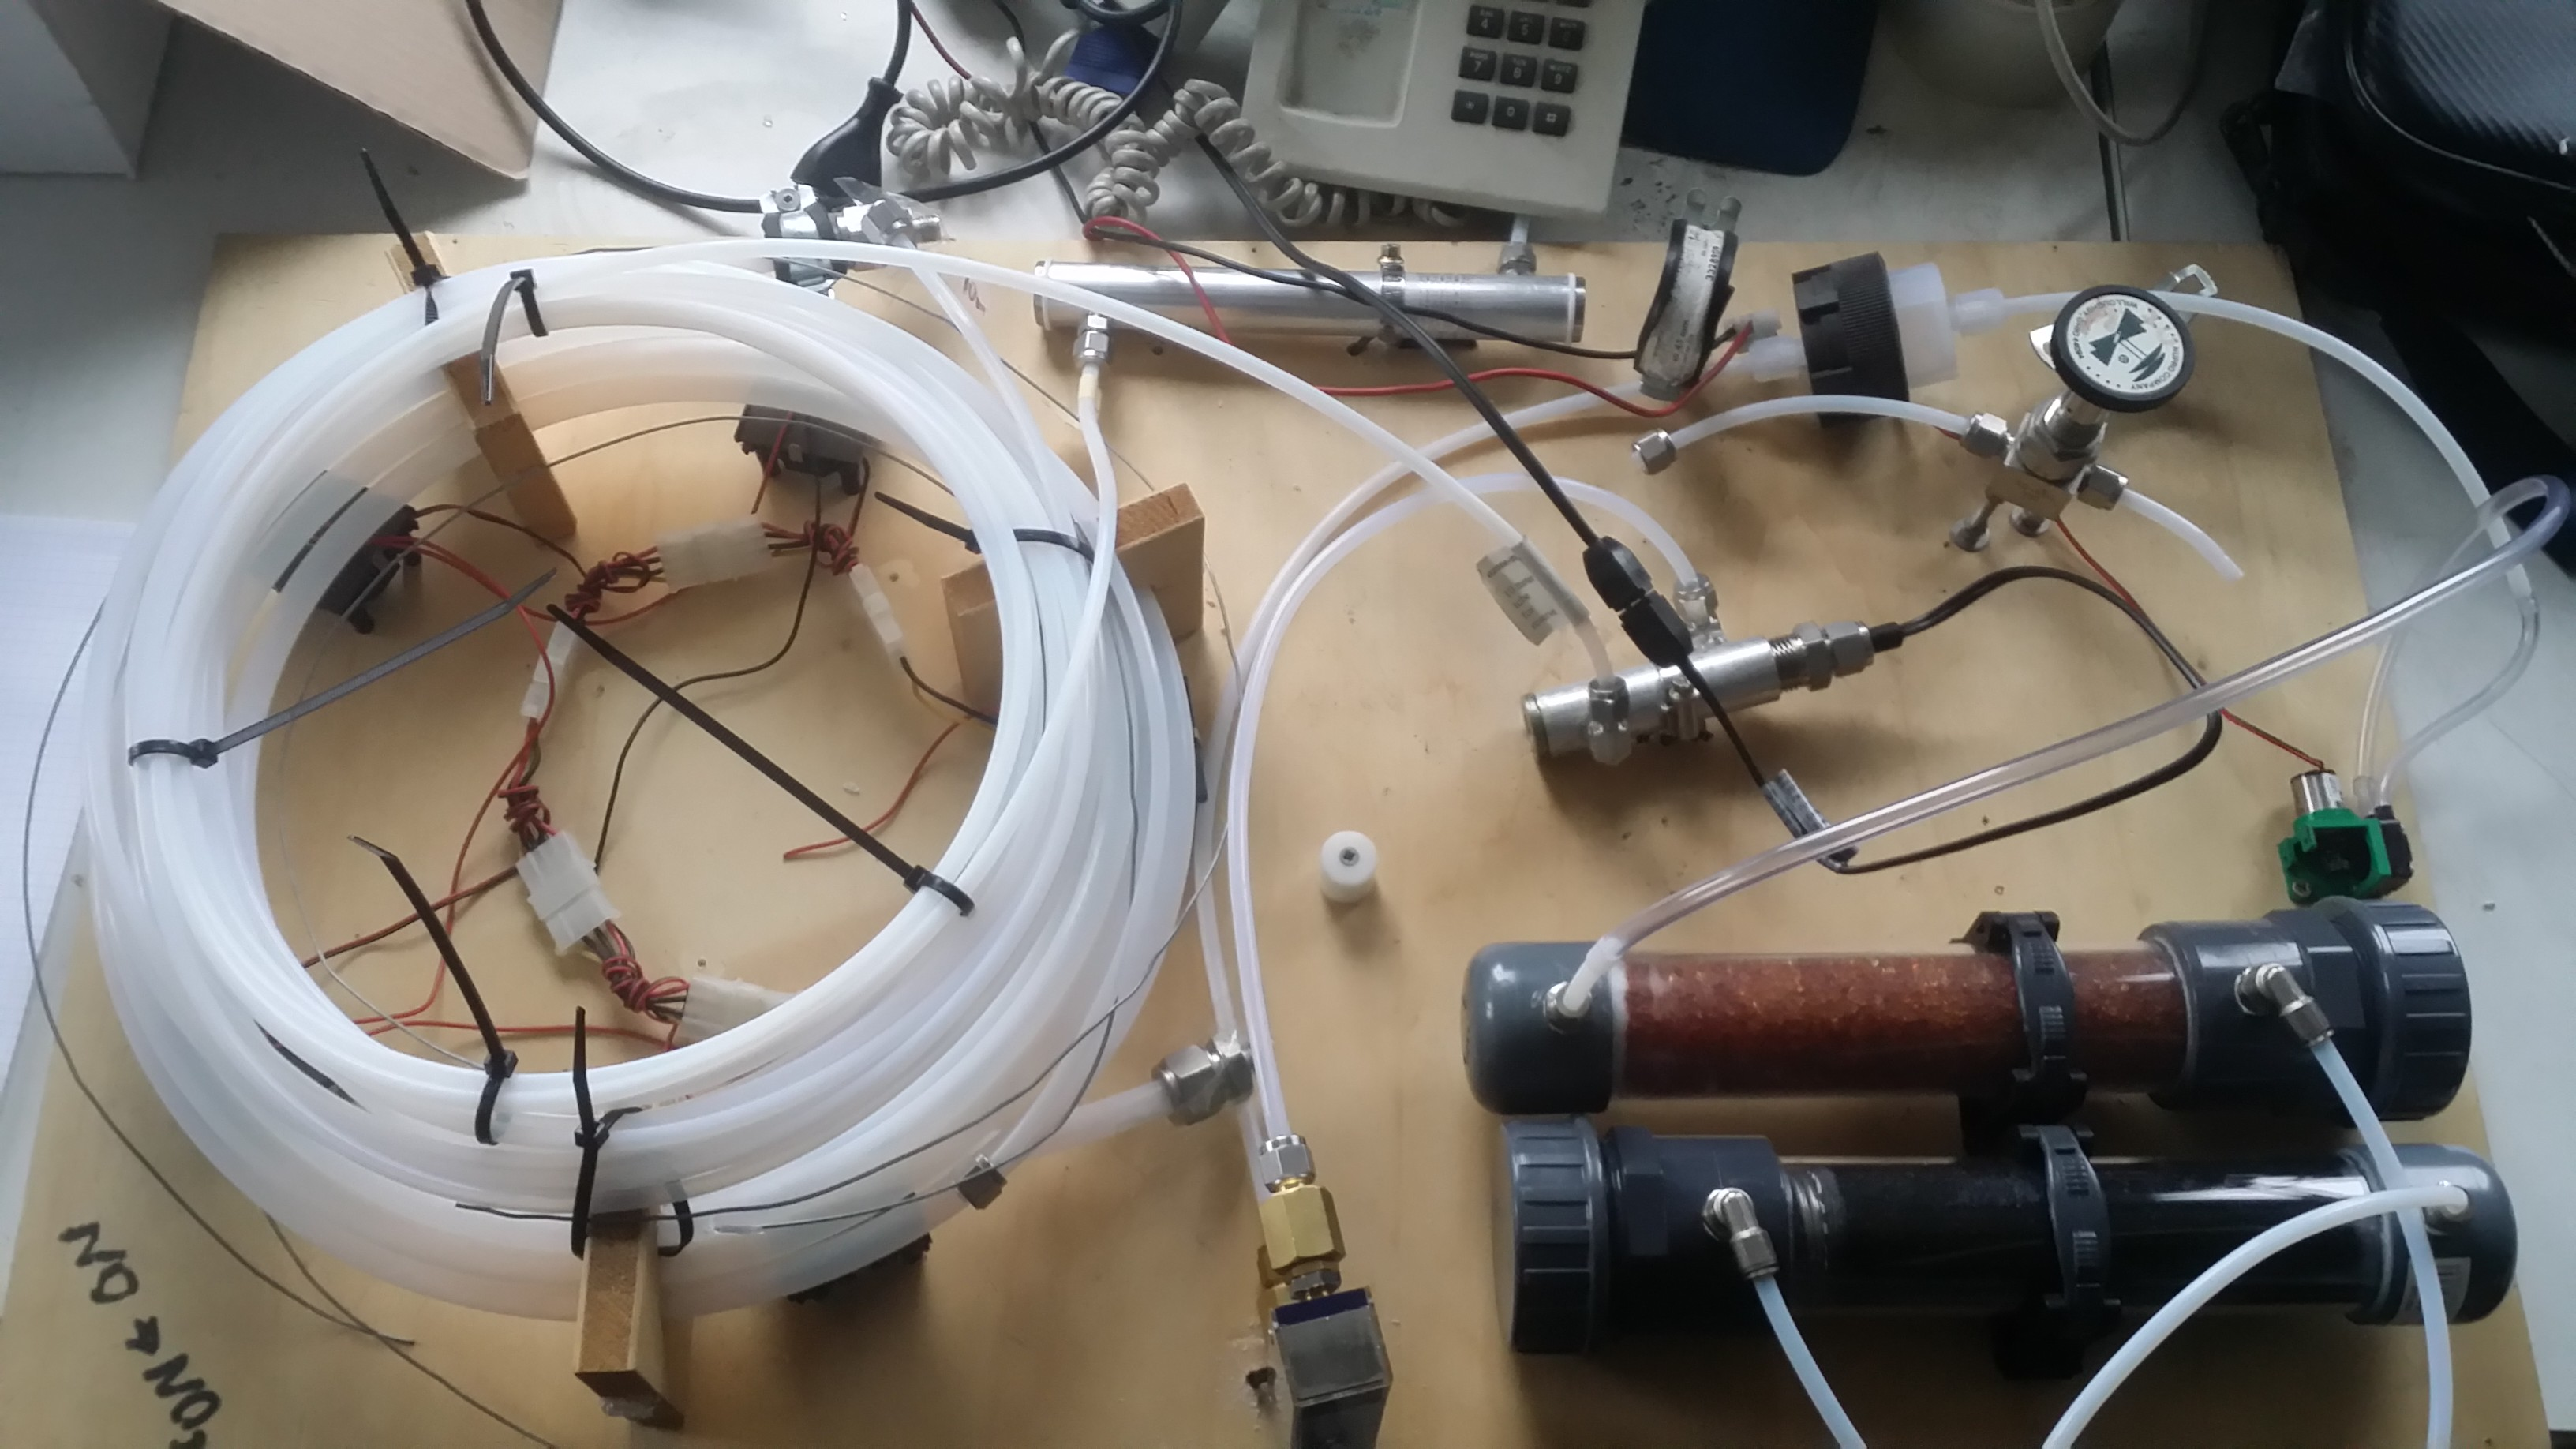
\includegraphics[width=\unitlength,page=1]{setup.pdf}}%
    \put(0.72339254,0.0272422){\color[rgb]{0,0,0}\makebox(0,0)[lb]{carbon filter}}%
    \put(0.68467052,0.20608212){\color[rgb]{0,0,0}\makebox(0,0)[lb]{\smash{silica gel}}}%
    \put(0.84485225,0.27636329){\color[rgb]{0,0,0}\makebox(0,0)[lb]{\smash{pump}}}%
    \put(0.66524548,0.47215208){\color[rgb]{0,0,0}\makebox(0,0)[lb]{\smash{particle filter}}}%
    \put(0.37854499,0.02340413){\color[rgb]{0,0,0}\makebox(0,0)[lb]{\smash{flowmeter}}}%
    \put(0.41093385,0.46876799){\color[rgb]{0,0,0}\makebox(0,0)[lb]{\smash{silica gel in tube}}}%
    \put(0.55474278,0.26558162){\color[rgb]{0,0,0}\makebox(0,0)[lb]{\smash{penray lamp in tube}}}%
    \put(0,0){\includegraphics[width=\unitlength,page=2]{setup.pdf}}%
    \put(1.00286136,0.04729665){\color[rgb]{0,0,0}\makebox(0,0)[lb]{\smash{lab air}}}%
    \put(0.59985726,0.5399915){\color[rgb]{0,0,0}\makebox(0,0)[lb]{\smash{ozone}}}%
    \put(0,0){\includegraphics[width=\unitlength,page=3]{setup.pdf}}%
  \end{picture}%
\endgroup%

%%% Local Variables:
%%% mode: latex
%%% TeX-master: "../Bachelor"
%%% End:

  }
  \phantom{h}\\
  \bigskip
  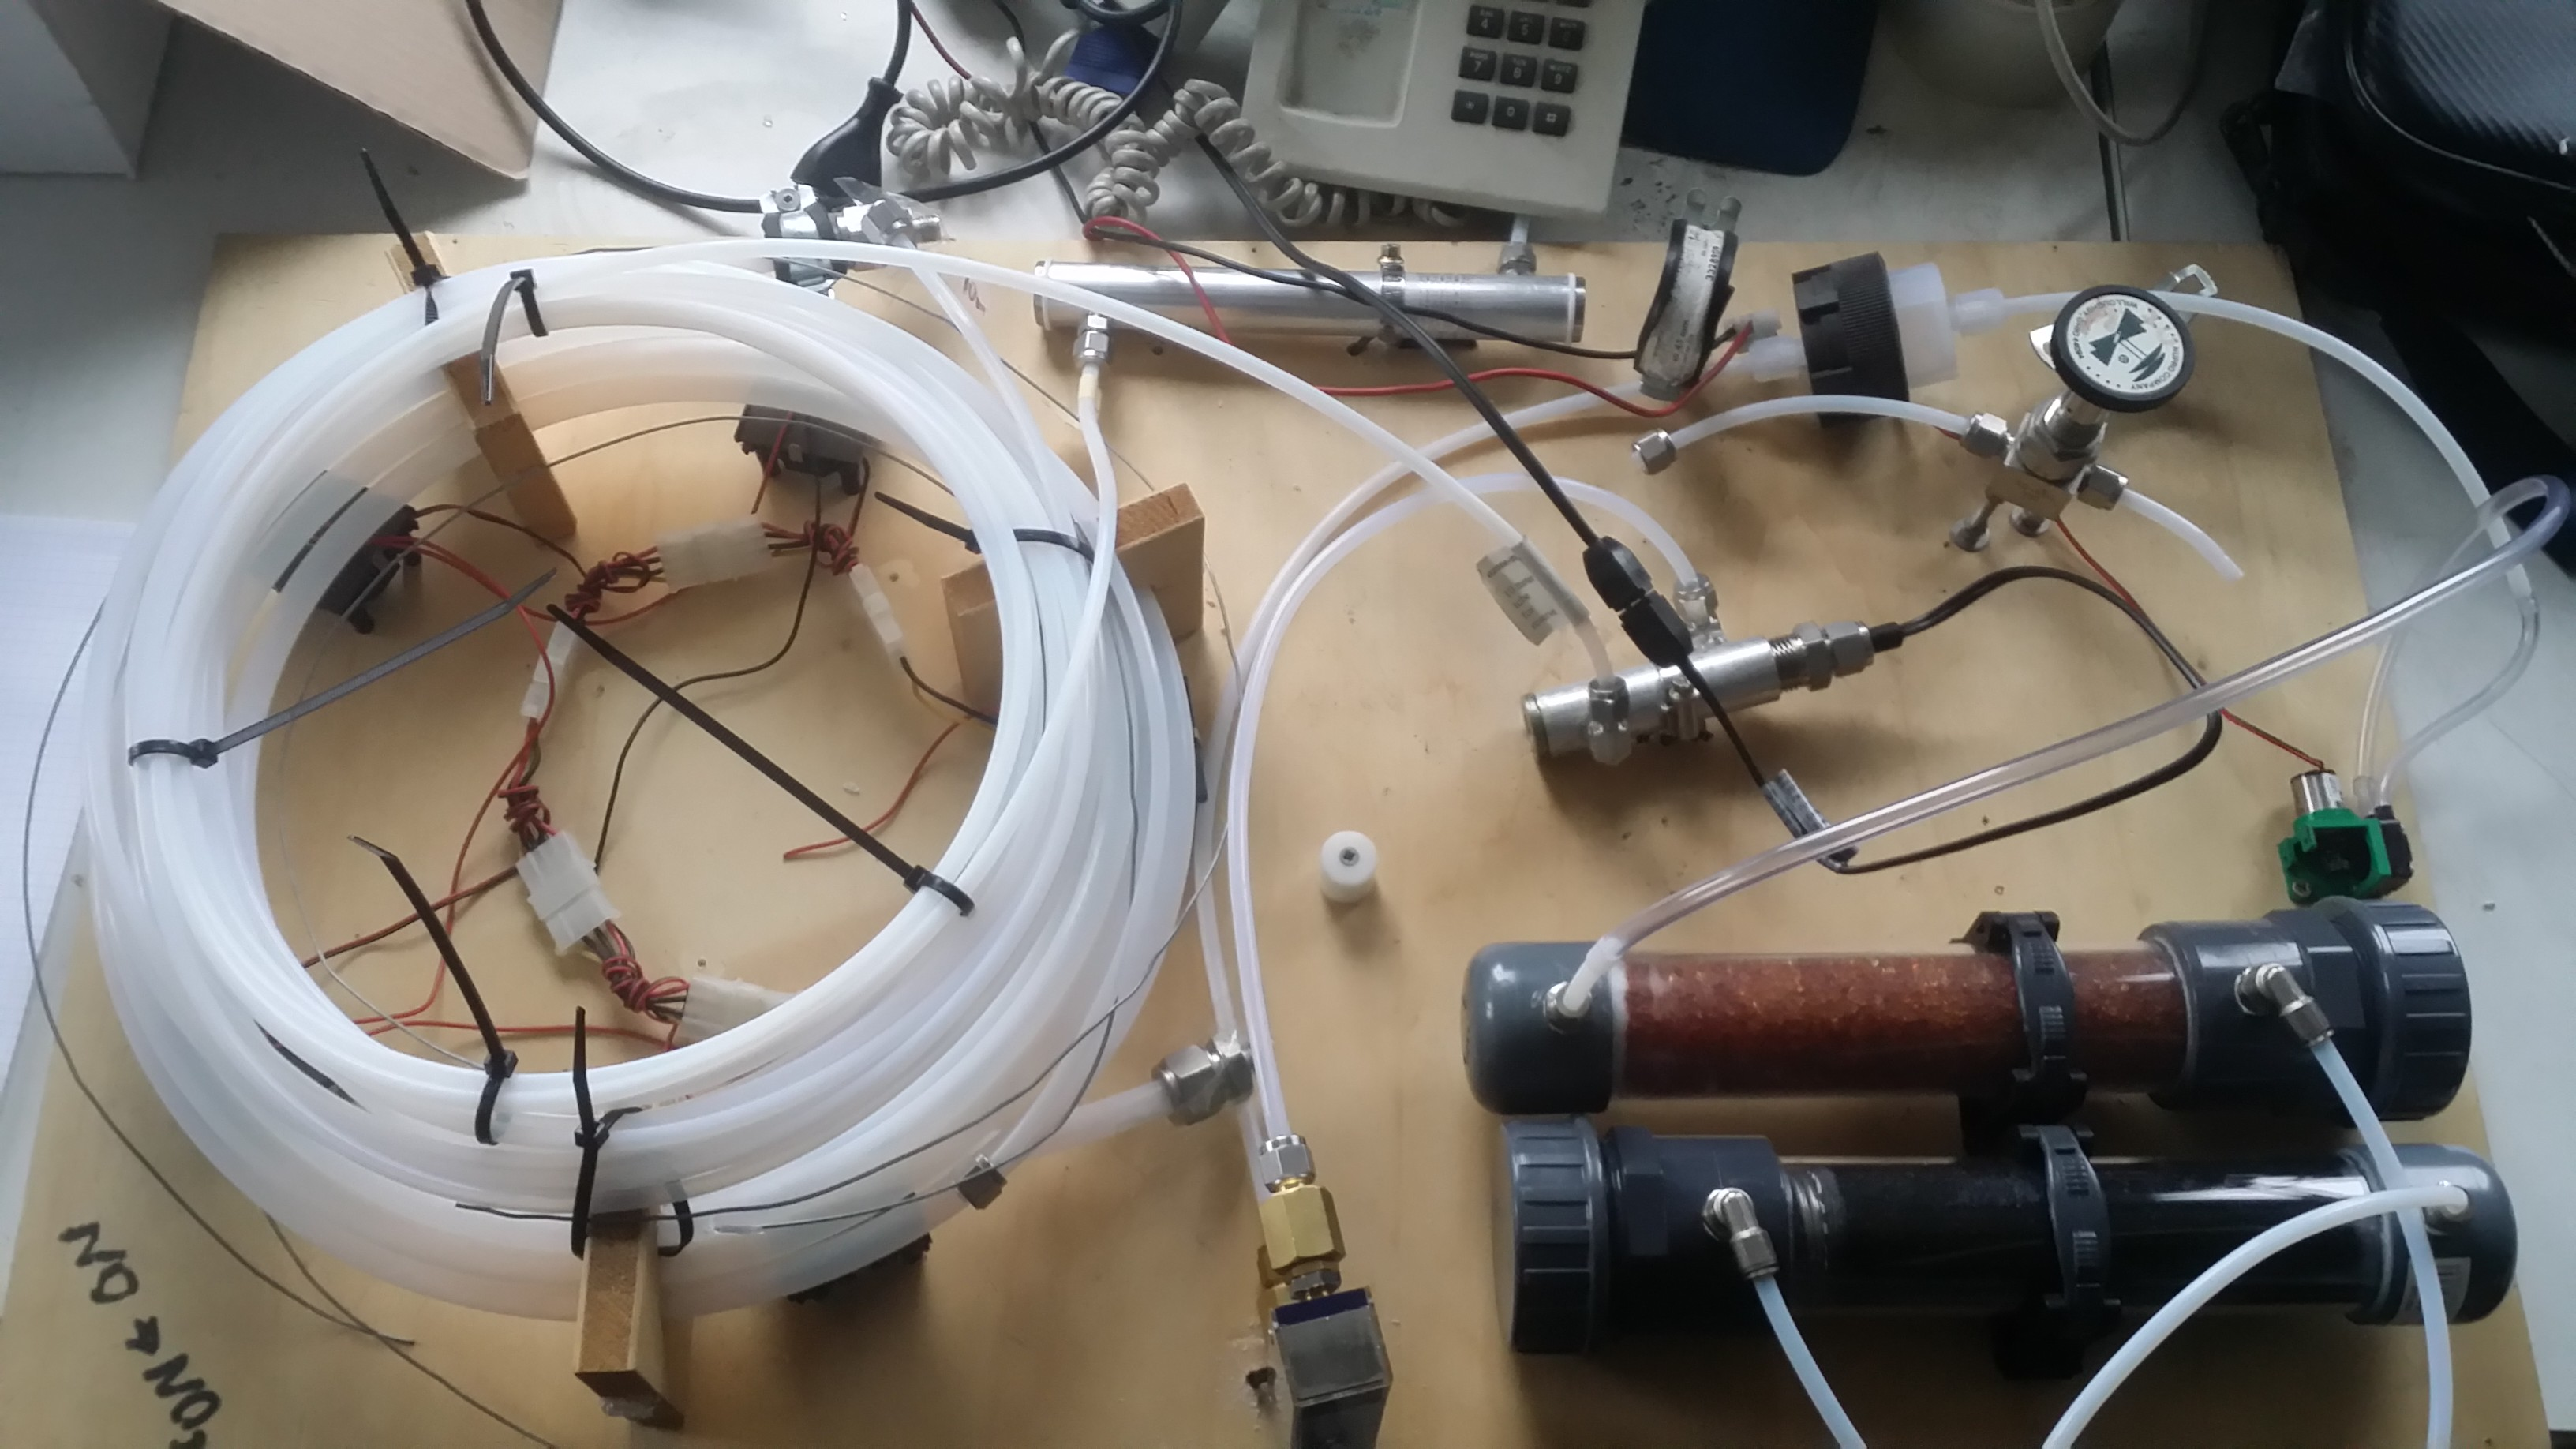
\includegraphics[width=0.9\linewidth]{setup.jpg}
  \caption{Ozone generator setup. Schematic and picture.}
  \label{fig:setup}
\end{figure}

The measurements are meant to answer the following questions:
\begin{itemize}
\item Does the Ozone pass the silica gel?
\item How much time does it take before the silica gel reaches the
  saturation level?
\item Depending on the power of the Penray lamp, how high is the Ozone
  concentration?
\item How much \ch{NO_x} is left in the air behind the generator?
\end{itemize}


\subsection{Measurements}
\label{sec:ozone-meas}

It is necessary to understand the characterstic of our instrument
before we use it to convert \ch{NO} to \ch{NO2}. For that we measured
the time it took to reach a stable production of Ozone and where this
level lay. 

In figure~\ref{fig:long-stop} one can see the time series of the Ozone
level of the generator, if the generator had been turned of for a long
time\footnote{In this case about a week.}. As can be seen the level
rises rather quickly and reaches a stable plateau after approximately
\SI{35}{\minute}. The equilibrium lies around 250ppm.

\begin{figure}[htbp]
  \centering
  \begin{tikzpicture}
    \begin{axis}[
      xlabel={Time [\si{\hour}]},
      ylabel={c(\ch{O3}) [ppb]},
      no markers,
      xmin=0,
      xmax=2,
      ]
      \addplot table [col sep=comma] {images/Anschaltkurve2.csv};
    \end{axis}
  \end{tikzpicture}
  \caption{Evolution of Ozone after a long full stop of the
    generator.}
  \label{fig:long-stop}
\end{figure}

In a next step we determined the time necessary to get back to the
equilibrium after shorter stops of the generator. For this we measured
the time series of the Ozone concentration after a stop of {\nfrac
  1/2} \si{\hour}, \SI{1}{\hour}, \SI{2}{\hour} and \SI{4}{\hour}. The
result can be found in figure~\ref{fig:multiple-stop}, which shows
that the Ozone reaches the saturation level within
\SI{10}{\minute}. That in this case the saturation level lay around
200 ppm can be explained by the difference in temperature between the
two measurements. 

\begin{figure}[htbp]
  \centering
  \begin{tikzpicture}
    \begin{axis}[
      xlabel={Time [\si{\minute}]},
      ylabel={c(\ch{O3}) [ppb]},
      legend entries={\nfrac 1/2\si{\hour}, \SI{1}{\hour}, \SI{2}{\hour},
        \SI{4}{\hour}},
      no markers,
      legend pos=south east,
      xmin=0,
      xmax=10,
      ]
      \addplot table [col sep=comma] {images/Multiple-stop.csv};
      \addplot table [col sep=comma,y=1h] {images/Multiple-stop.csv};
      \addplot table [col sep=comma,y=2h] {images/Multiple-stop.csv};
      \addplot table [col sep=comma,y=4h] {images/Multiple-stop.csv};
    \end{axis}
  \end{tikzpicture}
  \caption{Evolution of the Ozone concentration after a full stop of the
    generator.}
  \label{fig:multiple-stop}
\end{figure}

In a last step we researched the influence of a higher current at the
Penray lam on the Ozone level. Figure~\ref{fig:lamp} shows that after
turning on the lamp the saturation level rises from 200 ppm to over
350 ppm.

\begin{figure}[htbp]
  \centering
  \begin{tikzpicture}
    \begin{axis}[
      xlabel={Time [\si{\minute}]},
      ylabel={c(\ch{O3}) [ppb]},
      no markers,
      xmin=0,
      xmax=45,
      ]
      \addplot table [col sep=comma] {images/2015-12-02-current2.csv};
    \end{axis}
  \end{tikzpicture}
  \caption{Ozone level dependence on current of Hg-lamp.}
  \label{fig:lamp}
\end{figure}

\subsection{Ozone generator setting in a CE-DOAS instrument}
\label{sec:o3-setting-doas}

After installing the Ozone generator within a CE-DOAS instrument we
set up an experiment to test its wanted Ozone and its unwanted
\ch{NO2} production. The setup can be found in
Figure~\ref{fig:ozone-flow-setup}. We used to zero air catridges. One
at the zero air input (which also generates the Ozone) and one at the
sample air input. Thus the sample air is \ch{NO2} and \ch{O3}
free. The only way to find these trace gases is, if the Ozone
generater introduced them. Naturally we expect it to produce Ozone
however, we do not want it to produce Nitrogendioxide, which is why we
introduced a Silica filter after the generator. To test the effect of
this filter we took measurements with and without that filter at
different flows of the generator and checked the concentrations.

\begin{figure}[htbp]
  \centering
  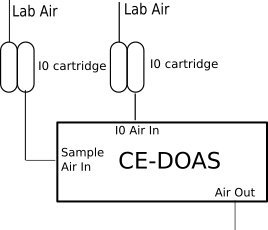
\includegraphics[width=0.35\textwidth]{ozone_setup.png}
  \caption{Ozone measurement setup}
  \label{fig:ozone-flow-setup}
\end{figure}

The result can be found in Figure~\ref{fig:o3-flow}. We see that
changing the flow ascendingly or descendingly does not have an
influence on the \ch{NO2} concentration as long as the silica filter
is in place. In both cases for flows smaller than
\SI{0.2}{\liter\per\minute} the concentration is practically
zero. Only at the very high flow of \SI{0.3}{\liter\per\minute} there
is \ch{NO2} detectable. The difference to the measurement without
Silica filter is obvious. Even the smallest stable flow leads to a
concentration of around \SI{4}{ppb} and for higher flows we soon reach
a stable plateau of about \SI{14}{ppb}. So we see that the Silica
filter is very effective in cleaning the generator air fo \ch{NO2}.

Looking at the Ozone levels we see a rise of the concentration with
the flow as is expected. On strange observation is that both
measurements \emph{with} Silica filter yield higher concentrations
than the measurment \emph{without} Silica filter. This seems
counterintuitive as the Silica gel should also filter some of the
Ozone before it reaches its saturation level. One possible explanation
might be that the silica gel adsorbs \ch{NO2} and other trace gases
fast enough such that they cannot react with the Ozone leading to a
higher Ozone concentration. \todo{Why is the ozone level without filter lower?}

\begin{figure}[htbp]
  \centering
  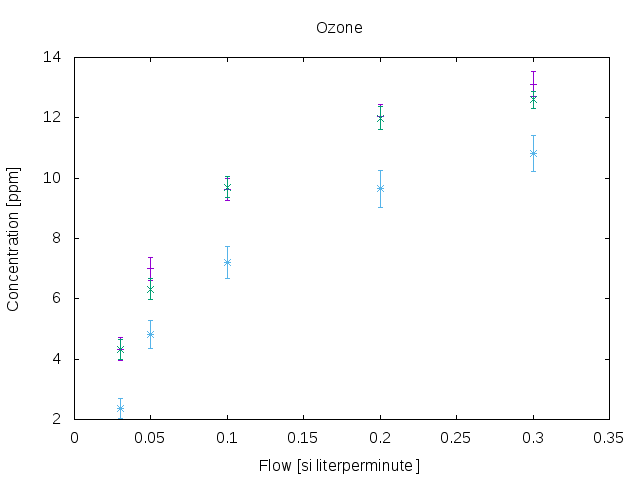
\includegraphics[width=0.45\textwidth]{O3.png}
  \hfill
  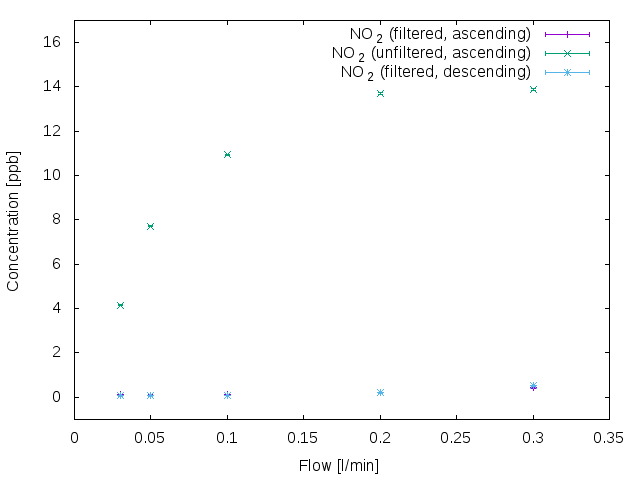
\includegraphics[width=0.45\textwidth]{NO2.png}
  \caption{\ch{O3} and \ch{NO2} concentration over generator flow.}
  \label{fig:o3-flow}
\end{figure}


%%% Local Variables: 
%%% mode: latex
%%% TeX-master: "../Bachelor"
%%% End: 
